There are still some features and optimizations that could be implemented to extend functionality, usability and reduce memory usage and CPU time.
This chapter addresses deflection plot accuracy, matrix data types, and dynamic system and stability analysis.

\section{Stability Analysis}
\label{sec:stabAna}

When the system contains non-trivial solutions a stability analysis could be performed to obtain the buckled shape by finding the eigenvalues

\begin{equation*} \label{eigenvalues}
det \lvert K + K_{geom} \cdot \lambda_n \lvert = 0 
\end{equation*}

and constructing the buckled shapes from $d$

\begin{equation*} \label{buckle}
( K + K_{geom} \cdot \lambda_n ) \cdot d = 0
\end{equation*}

\section{Dynamic Analysis}
\label{sec:dynAna}

A dynamic system analysis could be performed using member mass matrices $m$ 
\begin{equation} \label{strut3}
    m = \begin{bmatrix}
                   0 & 0		   & 0 & 0 & 0           & 0 \\
                     & \frac{m}{2} & 0 & 0 & 0           & 0 \\
                     &             & 0 & 0 & 0           & 0 \\
                     &             &   & 0 & 0           & 0 \\
                     &             &   &   & \frac{m}{2} & 0 \\
        Sym.         &             &   &   &             & 0
    \end{bmatrix}
\end{equation}

to assemble a global mass matrix $M$, obtain the eigenvalues

\begin{equation*} \label{eigenvalues2}
det \lvert K - \lambda_n \cdot M \lvert = 0 
\end{equation*}

and calculate the mode shapes

\begin{equation*} \label{modeshape}
(K - \lambda_n \cdot M) \cdot d = 0 
\end{equation*}

\section{Increasing Deflection Plot Accuracy}
\label{sec:deflplotaccu}

The model used here only provides deflection and rotation for the nodes (at the end of each element). To increase the resolution one could employ different tactics.
Namely, P-order (\cref{subsec:porder}) or N-order (\cref{subsec:norder}) increase.
However, a third approach was chosen here: approximation using cubic B\'{e}zier curves (\cref{subsec:bezier}).

\subsection{P-Order Increase}
\label{subsec:porder}

Increasing the P-order by using a higher order polynomial would require solving the underlying differential equation for every load type.
This wouldn't scale very well because load types would have to provide a suitable polynomial. Which would make it more complicated to add further load types. 

\subsection{N-Order Increase}
\label{subsec:norder}

The N-order increase is the most common method and used by almost every commercial software. It only requires a method to subdivide elements.
This lets the stiffness matrix grow very fast. But with the computing power and memory of current desktop PCs it only becomes an issue for very large systems.

\subsection{B\'{e}zier Curves}
\label{subsec:bezier}

A B\'{e}zier curve is a parametric curve with very convenient and intuitive properties. They are widely used in computer-aided design and engineering \cite[1.3]{beziercad} \cite[3.-5.]{bezier}.

The general definition is:

\begin{equation} \label{generalBezier}
B(t) = \sum\limits_{i=0}^n \binom{n}{i} (1-t)^{n-i} t^{i} P_i
\end{equation}

Here, a cubic B\'{e}zier curve ($n=4$) was used to approximate the deflection plot of an element. The curve is defined by four points $\{P_0, P_1, P_2, P_3\}$ where $P_0$ is the start and $P_3$ the end point. All four points create a bounding box.

The explicit form of the curve is:

\begin{align*} \label{cubeBezier}
B(t) = (1-t)^3 P_0 + 3 (1-t)^2 t P_1 + 3 (1-t) t^2 P_2 + t^3 P_3 && 0 \leq t \leq 1
\end{align*}

\begin{figure}[h]%
    \centering
    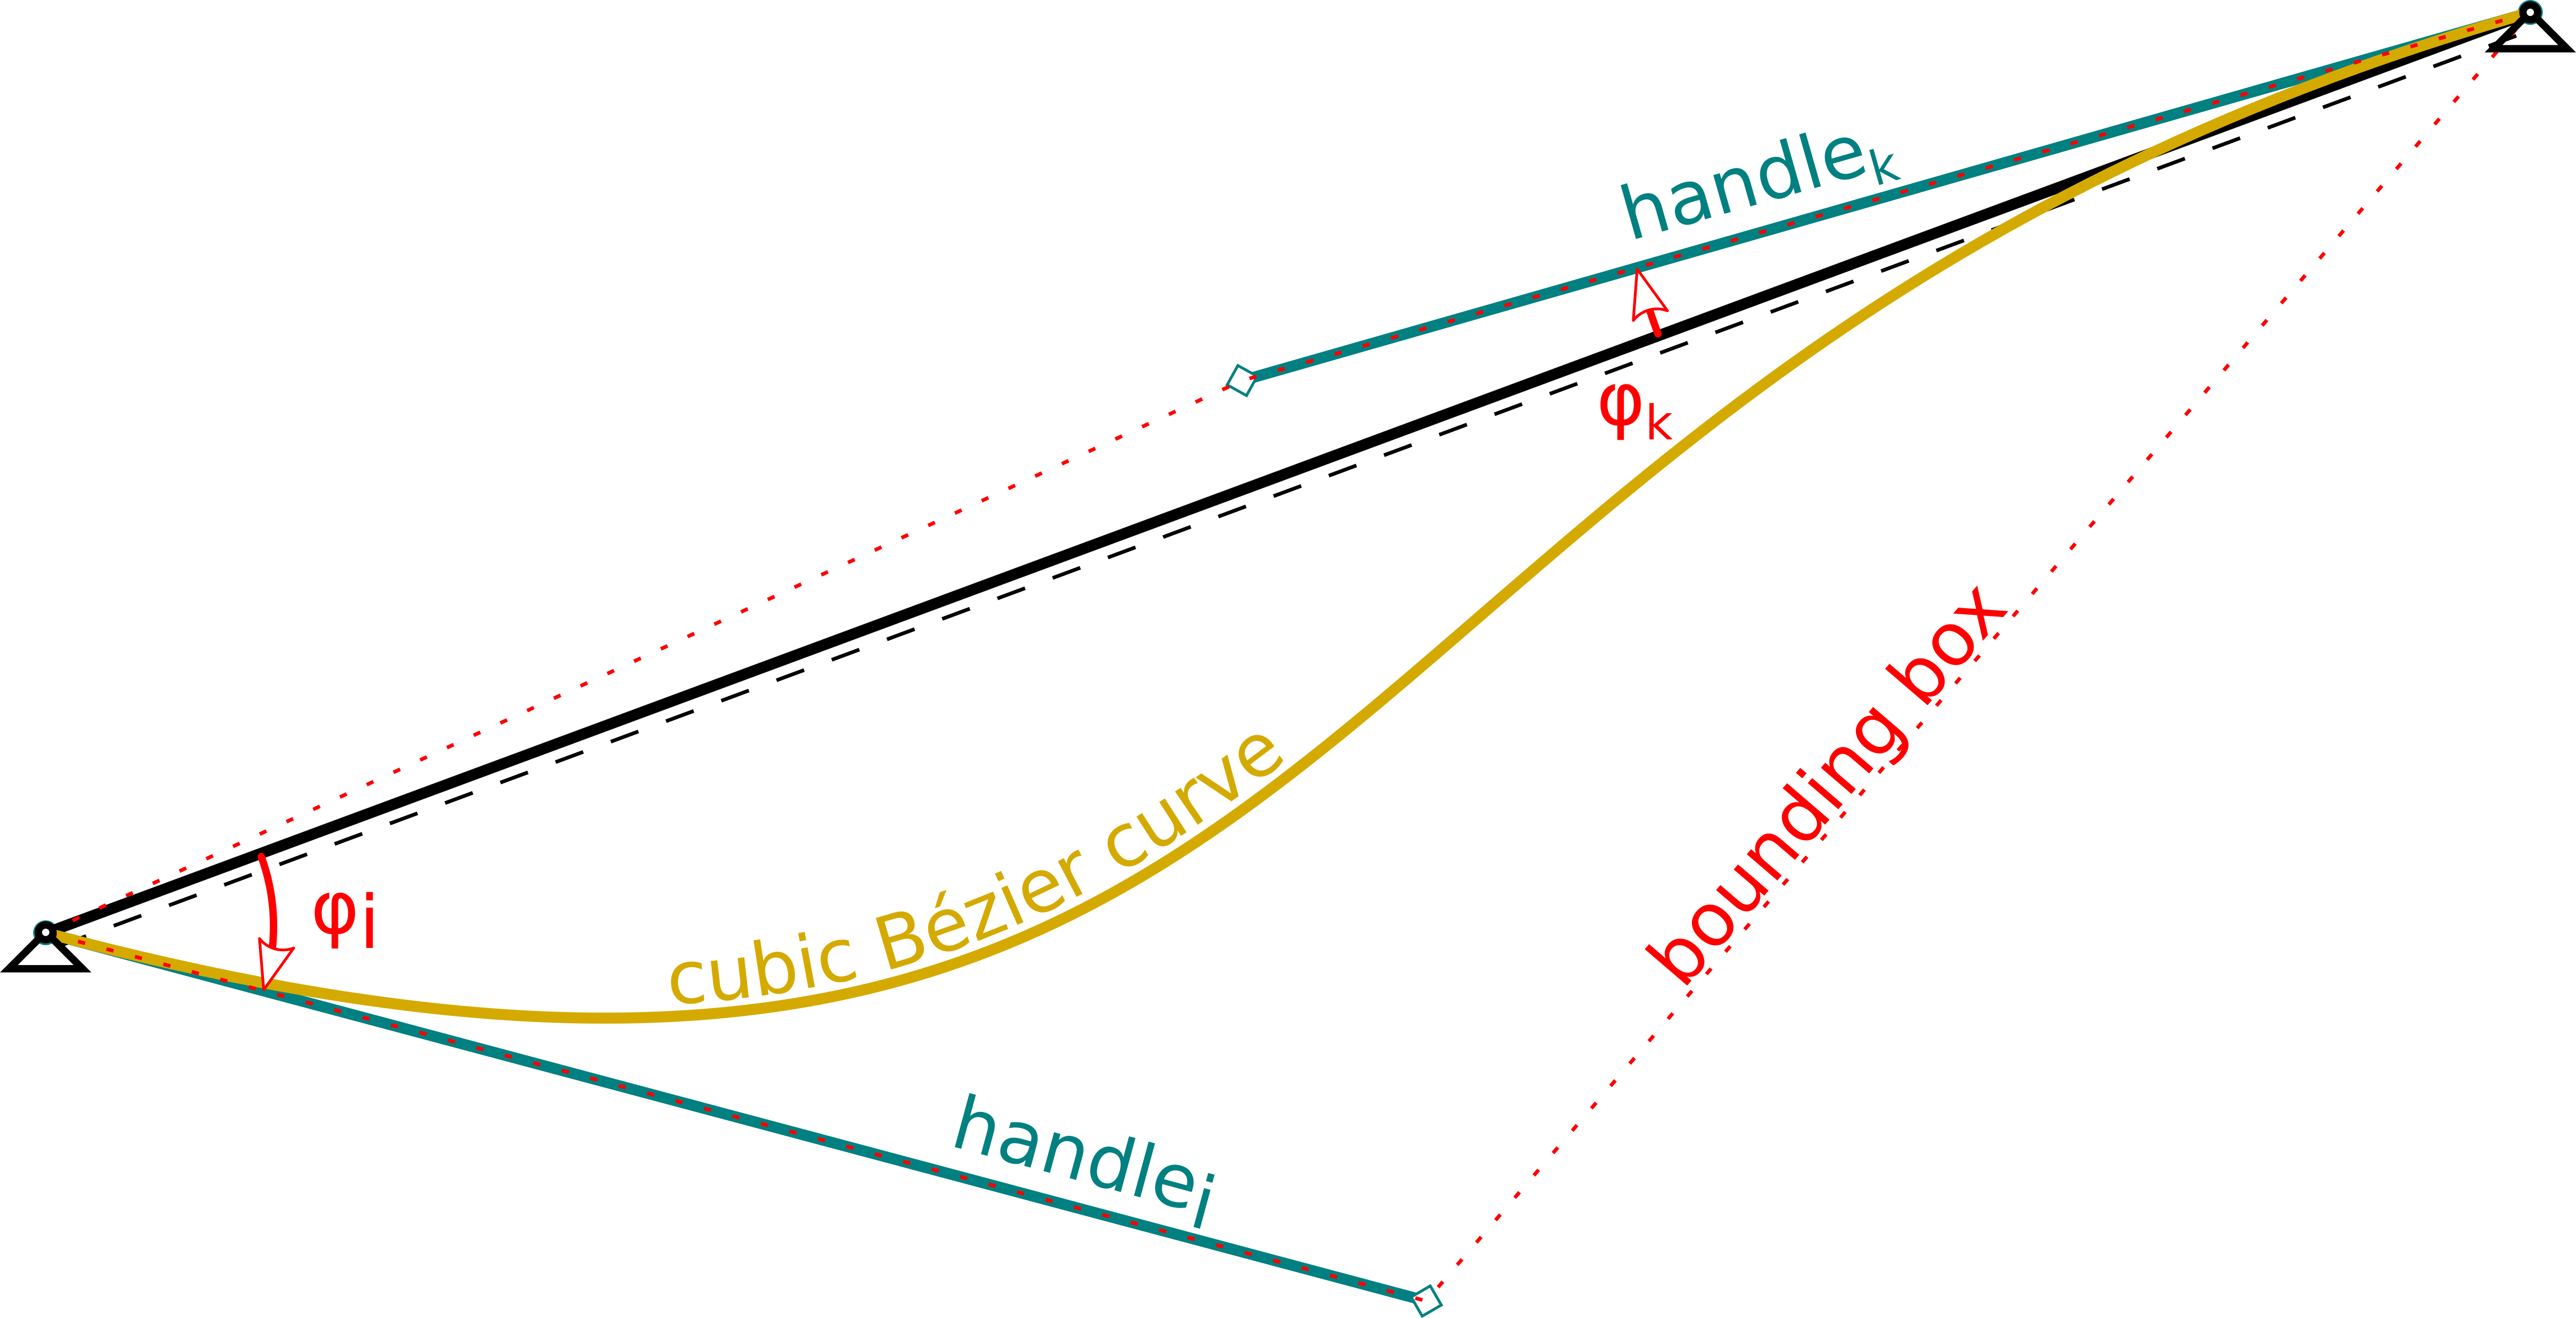
\includegraphics[width=0.9\textwidth]{cube_bezier.png}%
    \caption{Cubic B\'{e}zier curve}%
    \label{fig:cubeBezier}%
\end{figure}

The displacement and rotation at points $P_0$ and $P_3$ is known from the displacement vector $d$. Therefor the points are placed at:

\begin{equation*} \label{bezierHandles}
\begin{aligned}
P_0(x) &= node_n(x) + d_n^x \\
P_0(y) &= node_n(y) + d_n^y \\
P_3(x) &= node_{n+1}(x) + d_{n+1}^x \\
P_3(y) &= node_{n+1}(y) + d_{n+1}^y \\
\varphi_i &= d_n^r \\
\varphi_k &= d_{n+1}^r
\end{aligned}
\end{equation*}

In a first approximation the handle length ($\lvert\overrightarrow{P_0P_1}\lvert , \lvert\overrightarrow{P_3P_2}\lvert$) is set to one half of the strut length. This already turns out to produce qualitatively good results.
To increase accuracy even further, a relationship between handle length, stiffness and load could be developed but is not pursued in this thesis. 

\section{Sparse Matrix Data Type}
\label{sec:sparsematrix}

In this thesis the \textit{scipy} (\cref{sec:depend}) datatype \textit{ndarray} was used to store the matrices. This tracks all indices but the matrices are symmetric and even the global stiffness matrix $K_G$ (\cref{fullstiffnessmatrix}) only contains non-zero values three columns and rows above and below the diagonal.
A sparse matrix datatype like \textit{CSR} (Compressed Sparse Row Format) or \textit{COO} (Coordinate list) could be used to optimize for memory usage.
Or even a custom datatype that tracks only the indices containing non-zero values above the diagonal.
